\chapter{Clock Drift}\label{chap:6}
\minitoc

In the previous section, we introduced a timed automata model that 
describes a high level representation of systems execution. 
However, this type of model assumes that components clocks are perfectly synchronous which is 
hardly the case in practice.
Effectively, clocks are able to measure time up to a certain precision and will be likely
to drift since they are implemented based on oscillators that are not perfect: the oscillator 
frequency is not constant, it changes depending on environmental conditions such as 
temperature, humidity and aging.
Figure~\ref{fig:drift_exp} illustrates an example of two clocks $x$ and $y$ having different rate
with respect to an implicit perfect reference time. Figure (a) shows the case
where clock $x$ evolves steadily faster than clock $y$. Whereas, in Figure (b) 
clock $y$ is initially faster than clock $x$, then the trend is inverted after some time.

\begin{figure}[ht] 
\begin{minipage}[b]{0.5\linewidth}
\centering
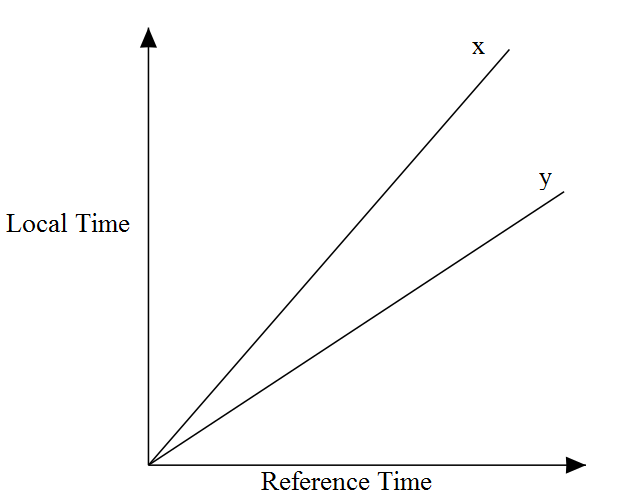
\includegraphics[scale=.55]{Figures/drift1}\\ 
  \vspace*{5mm} \small{(a)} 
\vspace{4ex}
\end{minipage}%%
\begin{minipage}[b]{0.5\linewidth}
\centering
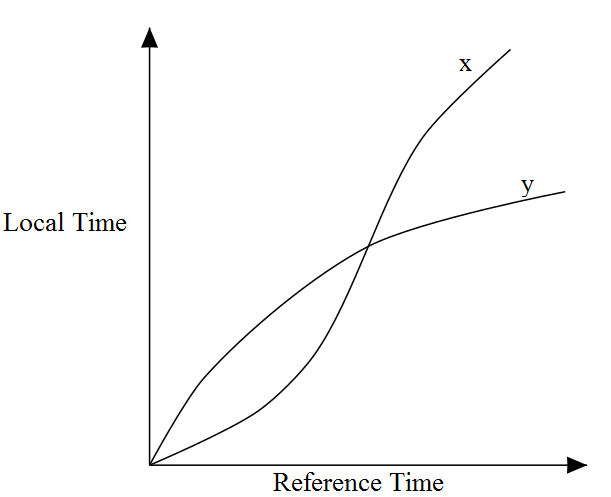
\includegraphics[scale=.55]{Figures/drift2}\\ 
  \vspace*{5mm} \small{(b)}
\vspace{4ex}
\end{minipage} 
\caption{Example of Clocks with Different Rates}
\label{fig:drift_exp}
\end{figure}

In this chapter, we present a distributed timed automata model where clocks advance at 
different rates and we study the resulting effect on the system behavior.

\section{Distributed Timed Systems with Independent Clock Rates}

\subsection{Expressing Clock Constraints Using Local Clock}

When building distributed real-time systems, a common practice is to use 
local clocks as time references as explained in Chapter~\ref{chap:3}.
These clocks measure the absolute time elapsed since the system startup and are never reset. 
This approach reduces the effort of keeping track of the actual time progress in components
and enable to have a common time scale. 

The idea consists in mapping each clock of a component to a (unique) local clock.
Thus, the value of component clocks are obtained by simply shifting their corespondent local 
clock by a constant amount of time as soon as the clocks are not reset.
Effectively, for each clock $x$ of a component, we introduce a real variable $\rho_x$ that 
stores the absolute time of its last reset (with respect to its local clock), that is, if $x$ 
is mapped to a local clock $g$, then each time $x$ is reset, $\rho_x$ is update to the current 
value of g.
Notice that the value of $x$ can be found by the equality $x=g-\rho_x$.
As a result, any timing constraints $c$ of a component $B_i$ can be expressed using a 
local clock $g$ as follows:
\begin{equation}
  \label{eq:glob}
  c = \bigwedge_{x_i\in\X_i} l\triangleleft x_i\triangleright u
    =\bigwedge_{x_i\in\X_i} l+\rho_{x_i}\triangleleft g\triangleright u+\rho_{x_i}
\end{equation}

where $\triangleleft\in\{<,\le\}$ and $\triangleright\in\{>,\ge\}$.
Notice any timing constraints of Definition~\ref{eq:cc} can be written on the form of 
inequalities. 


\subsection{Distributed Timed System}

Let $S=(\Loc,\loc_0,\X,\D,\gamma,\E_{\gamma},\{f_e\}_{e\in\gamma},\I)$ be a timed system of $n$ 
components synchronizing through the interaction set $\gamma$. 
For an interaction $\alpha$, we denote by $\clock{\alpha}$ the set of clocks appearing in its
timing constraints, that is, $\clock{\alpha}=\{x\in\X|\forall (\loc,\alpha,g,r,\loc')\in
\E_{\gamma}, x \ \circlled{$\in$} \ g \}$, with \circlled{$\in$} denoting the presence of
$x$ in the guard $g$.

Given an interaction partition $\{\gamma_k\}_{k=1}^m$, we put $\clock{\gamma_k}$ to denote
the set of clocks appearing in the timing constraints of interactions of $\gamma_k$, that is,
$\clock{\gamma_k}=\{\cup_{\alpha\in\gamma_k}\clock{\alpha}\}$.
We formalize the independent evolution of clocks by defining an \emph{ownership map} that assigns
a set of clocks to a unique local clock based on interaction partitioning . 
Particularly, we assign to each class of interaction a unique local clock. 
We require additionally that clock of each components is mapped only to a unique local clock.
This avoid timing inconsistency and ensure that each clock of a component is evaluated using 
a unique local 
clock. This constraints immediately the interaction partitioning as follows:
\begin{equation}\label{eq:tcf}
  \bigwedge_{\substack{i,j\in\{0,\cdots,m\}\\i\neq j}}\clock{\gamma_i}\cap\clock{\gamma_j}=
  \emptyset
\end{equation}

\begin{definition}[Distributed Timed System]\label{def:drft}
Given a timed system $S=(\Loc,\loc_0,\X,\D,\gamma,\E,$\\$\{f_e\}_{e\in\gamma},\I)$
and an interaction partitioning satisfying the constraint~\ref{eq:tcf}. 
We define the corresponding distributed timed system with independent local clock rates
as the tuple  
  $S^{dt}=(\Loc,\loc_0,\X^{dt},\D^{dt},\gamma,\E^{dt},\{f_e^{dt}\}_{e\in\gamma},\I^{dt},\pi)$ 
such that:
\begin{itemize}
  \item $\X^{dt}$ is the set of local clocks (a unique clock per class of interaction) 
  \item $\pi:\X\lto\X^{dt}$ is a many to one mapping between clocks $\X$ of $S$ and local clocks 
    $\X^{dt}$
  \item $\D^{dt}=\D\cup\{\cup_{x\in\X}\rho_x|\rho_x\in\realpoz\}$ is the set of data with 
    $\rho_x$ being real valued variables storing absolute reset times
  \item $\E^{dt}$ is such that for every $(\loc,\alpha,g,r,\loc')\in\E$, $\alpha\in\gamma$, we 
    have the corresponding transition $(\loc,\alpha,g^{dt},\emptyset,\loc')\in\E^{dt}$ where:
  \begin{itemize}
    \item $g^{dt}$ is the guard $g$ expressed using the local clock $x^{dt}\in\X^{dt}$ where
      $\forall x_i,x_j\in\clock{\alpha},i\neq j,\pi(x_i)=\pi(x_j)=x^{dt}$
    \item $f_e^{dt}=f_e\cup\{\rho_x:=x^{dt}|\forall x\in r\}$ is the transfer function updating 
      reset variables in addition to data variables of $\D$
  \end{itemize}
  \item $\I^{dt}$ is the set of location invariants expressed using local clocks 
\end{itemize}
\end{definition}

Notice that clocks appearing in location invariants appear necessarily in at least an 
interaction since we assume timed system with well formed guard.

\begin{property}[Semantics]
  The semantics of a distributed timed system $S^{dt}=(\Loc,\loc_0,\X^{dt},\D^{dt},$\\$\gamma,
  \E^{dt},\{f_e^{dt}\}_{e\in\gamma},\I^{dt},\pi)$ is defined by the timed transition system 
  $\ttsb{dt}=(\Q^{dt},q_0^{dt},\gamma,\lto_{\gamma})$ where:
  \begin{itemize}
    \item $\Q^{dt}=\Loc\times\V(\X_{dt}\cup\tcal{D}_{dt})\times\Delta$ where $\Loc$ is 
      the set of global locations, $\V(\X_{dt}\cup\tcal{D}_{dt})$ is the set of clock and 
      data valuations, and $\Delta=\real$ is the set offsets of local clocks in 
      $\X_{dt}$ with respect to an implicit (perfect) reference clock 
    \item $q_0^{dt}=(\loc_0,0,0)$ is the initial state.
    \item $\lto_{\gamma}\subseteq\Q^{dt}\times(\gamma\cup\realpos)\times\Q^{dt}$ is the set of 
      labeled transitions defined by the rules:
    \begin{itemize}
      \item $(\loc,\val,\delta)\transit{\alpha}_{\gamma}(\loc',\val[r],\delta)$ for 
        $\alpha\in\gamma$, if
      $(\loc,\alpha,g,r,\loc')\in\E^{dt}\wedge \val\models g$
    \item $(\loc,\val,\delta)\transit{d}_{\gamma}(\loc,\val',\delta')$ for $d\in\realpos$, 
      such that $\val'=\val+d-\delta+\delta'\wedge \val'\models\I^{dt}(\loc)\wedge\val'\ge\val$
    \end{itemize}
  \end{itemize}
\end{property}

The above semantics models drifting clocks by introducing an offset variable $\delta$ that 
stores for each clock in $x^{dt}$ its actual drift value with respect to an implicit 
reference time. The common practice when clocks are subject to drift is to
\emph{regularly resynchronize} the clocks using different methods, such as bit-stuffing 
or any other clock synchronization scheme.
Consequently, we consider a more realistic model where clocks can drift up
to a certain value $\epsilon$ with respect to a reference clock. This value is generally 
computed based on three parameters: \emph{(i)} the post-synchronization gap, \emph{(ii)} 
the longest gap between synchronizations, and \emph{(iii)} the clock precision parameter 
usually given by the constructor.
This induces that $\delta\in[-\epsilon,\epsilon]^{|\X^{dt}|}$.


\subsection{Properties}

\begin{property}\label{pr:rd}
  $\forall x,y\in\X^{dt},x\neq y,\delta=(\cdots,\delta_x,\cdots,\delta_y,\cdots)$
  where $|\delta|=|\X^{dt}|$, we have $\delta_x-\delta_y\in[-2\epsilon,2\epsilon]$
\end{property}

Property~\ref{pr:rd} states that the relative drift between local partitions 
clock is bounded by $2\epsilon$. This results from the fact that all local
clocks are kept within $\epsilon$ of a reference clock.

In order to attest the correctness of the distributed semantics, we compare
its corresponding time transition system ($\ttsb{dt}$) and the timed transition system 
of the standard semantics ($\ttsb{g}$).

Let $R$ be the relation:
\begin{align*}
  R=\{(q^{dt},q)\in\Q_{dt}\times\Q|q^{dt}=(\loc^{dt},\val^{dt},\delta), q=(\loc,\val) \\
  \text{ such that: }  
  \begin{cases}
  \loc^{dt}=\loc,\\
  \forall x\in\X,\val(x)=\valdt(\pi(x))-\rho_x-\delta_x  
\end{cases}
\end{align*}

The relation $R$ relates states of the distributed semantics with
states of the standard semantics having the same location configuration,
and whose clock valuations expressed on local clocks are $\delta\in[-\epsilon,\epsilon]$ close. 
We call such states $\epsilon-$similar.

\begin{lemma}\label{lem:equiv}
  For $\epsilon=0$, we have $\ttsb{dt}\sim_{R}\ttsb{g}$ 
\end{lemma}

Lemma~\ref{lem:equiv} describes the fact that a given system and its corresponding 
distributed model are bisimilar when $\Delta=0$, that is, when clocks advance at the same 
rate (perfect clocks). 

\begin{property}\label{pr:enabled1}
  Let $(\qdt,q)\in \RS$ such that $\qdt$ satisfies $\enabled{\alpha}$, then
  $q$ satisfies \\$\enabledbackwardb{\alpha}{0}{\epsilon}\vee\enabled{\alpha}
  \vee\enabledforwardb{\alpha}{0}{\epsilon}$.
\end{property}

Property~\ref{pr:enabled1} expresses that for states $(\qdt,q)\in\RS$ if it exists
an interaction enabled at $\qdt$ then this interaction is either enabled at $q$, 
will be enabled after a time progress of $\epsilon$ or is up to $\epsilon$ after 
the deadline of $\alpha$. This property flows directly from the $\epsilon-$similarity
of states $(\qdt,q)\in\RS$, the form of interactions timing constraints 
(conjunction of intervals)
and the fact that clocks involved in the same interaction advance at the same rate. 
It points out that any execution from
state $\qdt$ might not be always possible from state $q$ or any of its time successor.

\begin{lemma}\label{lm:enabled1}
  Let $(\qdt,q)\in\RS$ such that $\qdt$ satisfies $\enabled{\alpha}\wedge
  \enabledbackwardb{\alpha}{\epsilon}{\epsilon}$, then
  $q$ satisfies $\enabledbackwardb{\alpha}{0}{\epsilon}$.
\end{lemma}
Lemma~\ref{lm:enabled1} can be deduced straightforwardly from property~\ref{pr:enabled1}.
It expresses that for states $(\qdt,q)\in\RS$, if it exists an interaction $\alpha\in\gamma$
such that $\alpha$ is enabled at $\qdt$ and that clock valuations are up to $\epsilon$ 
before the deadline of this interaction then, $\alpha$ can be executed from $q$ or any of its 
$\epsilon-$time successors (by doing a time progress up to $\epsilon$).

The usual notion of simulation as defined in~\ref{def:sim} is too precises. 
It requires that each trace in one system
can be matched~\emph{exactly} by a trace in the other system, that is, 
two states can be distinguished even for an infinitesimally
small mismatch between timings ($\epsilon\neq0$). 
Thus, we rely on the following quantitative variant of simulation~\cite{drift:esim}. 

\begin{definition}[$\epsilon-$simulation]\label{def:esim}
  Given two TTS, $\TTSc{1}$ and $\TTSc{2}$, a relation $R\subseteq\Q_1\times\Q_2$ is a:
  \begin{itemize}
    \item Strong timed $\epsilon-$simulation, if for any $(q_1,q_2)\in R$, $\sigma\in\sum$, 
      $d,\epsilon\in\realpoz$
    \begin{itemize}
      \item $q_1\transit{\sigma}\q_1'$ implies $q_2\transit{\sigma}q_2'$ for some $q_2'\in\Q_2$ 
        with $(q_1',q_2')\in R$
      \item $q_1\transit{d}\q_1'$ implies $q_2\transit{d'}q_2'$ for some $q_2'\in\Q_2$ and 
        $d'\in\realpoz$ with $|d'-d|\le\epsilon$ and $(q_1',q_2')\in R$
    \end{itemize}
    \item Timed action $\epsilon-$simulation, if for any $(q_1,q_2)\in R$, $\sigma\in\sum$, 
      $d,\epsilon\in\realpoz$
    \begin{itemize}
      \item $q_1\transit{d,\sigma}\q_1'$ implies $q_2\transit{d',\sigma}q_2'$ for some $q_2'
        \in\Q_2$ and $d'\in\realpoz$ with $|d'-d|\le\epsilon$ and $(q_1',q_2')\in R$
    \end{itemize}
  \end{itemize}
  If there exists a strong timed (resp. timed action) $\epsilon-$simulation
  between $\ttsb{1}$ and $\ttsb{2}$ w.r.t $R$, then we write
  $\ttsb{1}\sqsubseteq^{\epsilon}_{R}\ttsb{2}$ (resp. $\tts{1}\sqsubseteq^{\epsilon*}_{R}
  \ttsb{2})$
\end{definition}


This approach characterizes
the degree of closeness between timed systems: it generalizes the (boolean) 
notions of timed simulation
(yes or no) to metrics over timed system. Formally, for a positive real number
$\epsilon$, a state $q_1$ is 
told $\epsilon-$similar to another state $q_2$ if there is a time-abstract simulation 
that can relates both states in
the sense that the difference between the delays of time-step transitions is at most $\epsilon$.

Although this definition of simulation is less 
restrictive, Property~\ref{pr:enabled1} gives the intuition that for some states
$(\qdt,q)\in\RS$ there may be interactions that can be executed from $\qdt$ but not from
$q$, which make the $\epsilon-$simulation impossible.

\section{Robust Distributed Semantics}
As explained in previous sections, the distributed semantics may 
exhibit new behavior with respect to the standard semantics.  
In this section, we identify the problematical states of the 
distributed semantics and provide sufficient conditions
that will guarantee timed action $\epsilon-$simulation. 

\begin{definition}[Potentially Bad States]\label{def:pbss}
  We denote by $\Upsilon$ the set of potentially bad states of the 
  distributed semantics characterized as follows:
  \[\Upsilon=\{q=(\loc,\val)|\exists\alpha\in\gamma,\val\models g_{\alpha}\wedge
  \val+\epsilon\not\models g_{\alpha} \} \]
\end{definition}

The intuition behind this characterization results form Property~\ref{pr:enabled1}.
These states may yield possible execution of interactions in the distributed semantics that
are not possible in the related states of the standard semantics (states that are 
$\epsilon-$similar). 

\begin{proposition}\label{prop:esim}
  Let $\ttsb{dt}$ be the timed transition system of the distributed semantics. 
  We have: 
  \[\Upsilon\cap\reach^*(\ttsb{dt})=\emptyset\implies\ttsb{dt}\sqsubseteq^{\epsilon*}_{\RS}
  \ttsb{g}\]
  where $\reach^*(\ttsb{dt})$ is the projection of states of the distributed semantics 
  on state variables of the standard semantics, that is, by considering only locations, clocks,
  and data variables.
\end{proposition}

\begin{proof}[Proof of Proposition~\ref{prop:esim}]
  
  In order to prove proposition~\ref{prop:esim}, we need to show that if for any 
  $(\qdt,q)\in\RS$, $\sigma\in\gamma$ and $d\in\realpoz$:
      \begin{displaymath}
        \qdt\transit{d,\sigma}\qdtb \implies \exists q'\in\Q^g, q\transit{d',\sigma}q',
        \text{ with } 
        d'\in\realpoz, \ |d'-d|\le\epsilon \text{ and } (\qdtb,q')\in\RS
      \end{displaymath}
       
      Let $(\qdt,q)\in\RS$ such that $\Upsilon\cap\reach^*(\ttsb{dt})=\emptyset$ and 
      $\exists\sigma\in\gamma,\exists d\in\realpoz,$ 
  $\qdt\transit{d,\sigma}\qdtb$. We distinguish two cases:
  \paragraph{\textbf{Case 1: $d > 0$}\\}
  We have $\qdt \transit{d,\sigma}\qdtb$. This means:
    \[
    \begin{cases}{}
      \valdtb=(\valdt+d-\delta+\delta')[r^{dt},f_{\sigma}] \\  
      \valdt +d-\delta+\delta'\models\I^{dt}(\loc)\wedge g_{\sigma}^{dt} \\ 
      \valdt +d-\delta+\delta'+\epsilon\models\I^{dt}(\loc)\wedge g_{\sigma}^{dt}& 
      \qdt\notin\Upsilon 
    \end{cases}\]
  where $[r^{dt},f_{\sigma}]$ means after applying reset and transfer function.
  When expressed on original clocks the above becomes:
    \[\begin{cases}{}
      \valdtb=(\val+\rho+d+\delta')[r^{dt},f_{\sigma}]\\ 
      \val+d+\delta'\models\I(\loc)\wedge g_{\sigma} \\ 
      \val+d+\delta'+\epsilon\models\I(\loc)\wedge g_{\sigma} 
    \end{cases}\]
  We also have $\delta'\in[-\epsilon,\epsilon]$. Consequently we have: 
  
  \begin{enumerate}
    \item $\delta'\in[0,\epsilon]$, then:\\
      \[\begin{cases}{}
        \valdtb=\val+d+\delta'+(\rho)[r^{dt},f_{\sigma}]\\ 
      \val+d+\epsilon\models\I(\loc)\wedge g_{\sigma} \label{1} 
    \end{cases}\]
    By putting $d'=d$, and  since $r^{dt}=\emptyset$ (Definition~\ref{def:drft}) and 
      $f_{\sigma}$ applies only on $\rho$ we obtain: 
      \[\begin{cases}
        \valdtb=\val+d'+\delta'+(\rho)[r^{dt}] \\ 
      \val+d'+\epsilon\models\I(\loc)\wedge g_{\sigma} \label{1} 
      \end{cases}\]%%%%%
      Consequently, we can conclude that $q\transit{d',\sigma}q'$ such $(\qdtb,q')\in\RS$
    \item $\delta'\in[-\epsilon,0]$, then:\\
      \[\begin{cases}{}
        \valdtb=\val+d+\delta'+(\rho)[r^{dt},f_{\sigma}]\\ 
      \val+d-\epsilon+\epsilon\models\I(\loc)\wedge g_{\sigma} \label{1} 
    \end{cases}\]
    By putting $d'=d$, and  since $r^{dt}=\emptyset$ (Definition~\ref{def:drft}) and 
      $f_{\sigma}$ applies only on $\rho$ we obtain: 
      \[\begin{cases}
        \valdtb=\val+d'+\delta'-\epsilon+(\rho)[r^{dt}] \\ 
      \val+d'\models\I(\loc)\wedge g_{\sigma} \label{1} 
      \end{cases}\]%%%%%
      Consequently, we can conclude that $q\transit{d',\sigma}q'$ such $(\qdtb,q')\in\RS$
  \end{enumerate}
  
  \paragraph{\textbf{Case 2: $d = 0$}\\}
   Since $\Upsilon\cap\reach^*(\ttsb{dt})=\emptyset$, using the same methodology of case 1, 
   we can conclude that $\exists q'\in\Q^g, q\transit{d',\sigma}q',\text{ with } 
        d'\in\realpoz, \ |d'-d|\le\epsilon \text{ and } (\qdtb,q')\in\RS$.
\end{proof}

Proposition~\ref{prop:esim} highlights an interesting property on the reachable states of the 
distributed semantics. It states that if all the reachable states of the 
distributed semantics are not potential bad states, i.e, $\Upsilon\cap\reach^*(\ttsb{dt})=
\emptyset $, then there exists a timed action $\epsilon-$simulation between the timed transition 
systems of the standard semantics and the distributed semantics.

Consequently, the idea is to restrict the distributed semantics in order to
avoid such states. 
This can be achieved by shrinking the upper bound of every transition timing constraints, if it 
exists, by $\epsilon$.   
Let $\ttsb{\dte}$ be the timed transition system after shrinking every existing upper bound timing
constraints by an amount of $\epsilon$. Then, we have the following lemma:
\begin{lemma}
  $\ttsb{\dte}\subseteq\ttsb{dt}$
\end{lemma}
The above lemma derives straightforwardly from the fact that shrinking does not introduce new
behavior. Conversely, it just restrains the set of states from which interactions can be 
executed.

\begin{lemma}\label{lem:shrink}
  $\Upsilon\cap\reach^*(\ttsb{\dte})=\emptyset$.
\end{lemma}
The above lemma is a direct consequence of the shrinking operation.   
In fact, since clocks of the distributed semantics an those of the standard semantics can have
at most $\epsilon$ difference in values, by shrinking upper bound timing constraints we avoid
all possible execution of interactions for clock values that are $\epsilon$ before its due date.
Consequently, this ensures that $\Upsilon\cap\reach*(\ttsb{\dte})=\emptyset$ and allows for any 
related state of the standard semantics to execute the same interaction
directly or after doing a timed step. 
%This can be effectively achieved by restricting the progress of time based to 
%$\epsilon$ before the due date of interactions.
%Preventing the progress of time $\epsilon$ time units
%before any interaction deadline will prevent any execution not possible 
%in the corresponding state of the standard semantics.
%Formally, this restriction can be written as follows:
%\begin{equation}\label{eq:res}
% (\loc,\val,\delta)\transit{d}_{\gamma}(\loc,\val',\delta') \text{ for } d\in\realpos, 
%      \text{ such that }\val'=\val+d-\delta+\delta'\wedge \val'\models\I(\loc)\wedge
%      (\loc,\val',\delta')\notin\Upsilon
%\end{equation}

%The above restriction of time progress helps to avoid reaching the potential bad states
%characterized by Definition~\ref{def:pbss}. However, this restriction does not guarantee 
%the non-reachability of such states. In fact, interaction executions may as well lead 
%to state of $\Upsilon$. Consequently, to prove that any reachable state of the distributed
%semantics is not a potentially bad state, we need to ensure that any \emph{arrival state},
%that is, state reachable immediately after the execution of an interaction is not a potentially
%bad state.
The following lemma is a direct consequence of Proposition~\ref{prop:esim} and Lemma~\ref{lem:shrink}.
\begin{lemma}
  $\ttsb{\dte}\sqsubseteq^{\epsilon*}_{\RS}\ttsb{g}$
\end{lemma}

\begin{definition}[Robustness]\label{def:rob}
  For a given timed system S, we say that S is robust to clock drifts iff $\reach(\ttsb{\dte})$ 
  is deadlock free.
\end{definition}

Restricting the distributed semantics through shrinking allows to avoid the reachability of some states 
(the potential bad states). This enforces the timed action $\epsilon-$simulation between states
of the standard semantics and those of the restricted distributed semantics.
However, since shrinking reduces the set of reachable states, the timed action $\epsilon-$simulation
alone is not enough. We must also ensure that shrinking does not introduce any deadlocks. 
The two aforementioned point together form our definition of robustness.

\section{Discussion}

In this chapter, we revisited the robustness concept usually used to check whether a given
system still satisfies the specification (a set of properties) when subject to different
perturbations such as clock drift. We first modeled the behavior of a timed system with 
independent clock rates and subject to a resynchronization scheme. Thereafter, we used
a variant of simulation that relates states with a timing difference up to a certain $\epsilon$,
and provide a characterization of potential bad states that may invalidate this variant of 
simulation. Then, we suggested a strategy based on shrinking upper bound timing constraints
in order to avoid such states which allows to attest the timed action $\epsilon-$simulation.

Sankur et al.~\cite{ocan} studied the robustness problem in timed automata against guards
shrinking. They provided a method for deciding whether shrinking all timing constraints (guards)
of a timed automaton, by possibly different amounts, results in a timed automaton that 
preserves some time-abstract behaviors, and is not blocking. The latter represents their
robustness notion.
It was proven that if the automaton is shrinkable, then several properties established on the 
initial automaton are preserved in the implementation (when clocks are not perfect). 
Otherwise, then the conclusion is that the model is vulnerable to the slightest variations in the 
measure of time and should thus be considered as non-robust, and the design should be reviewed.
From a theoretical aspect, the proposed analysis was formulated as a parameter synthesis
problem. \texttt{Shrinktech}~\cite{ocan2} is a tool that implements the simulation-shrinkability 
algorithm presented in~\cite{ocan}. It is compatible with the Kronos~\cite{kronos} model checker,
that can minimize the region graph of a timed automaton~\cite{tl} needed by the tool.
The tool has been used to attest the shrinkability of several case studies, such as 
the Philips Audio Retransmission protocol, Fischer's Mutual
Exclusion protocol (up to 4 agents), and some other asynchronous circuit models.
These experiments showed that the tool is capable of treating shrinkability of timed automata 
with thousands of edges (w.r.t graphs with more than sixty thousand transitions).
The bottleneck of the tool was also identified as being the size of the full bisimilarity graph,
which is often costly to compute, and that may require long processing time for shrinkability analysis. 
Moreover, the non-shrinkability of most models was mainly due equality constraints, or to the fact
that some models was designed at a high level of abstraction where imprecisions were
not taken into account.




